\chapter{ LIMBERO-GRIEEL, Controller Tuning}
\label{ch:chapter_six}

This chapter discusses the last step in setting up simulations and experiments on LIMBERO-GRIEEL. 
In chapter \ref{ch:chapter_four} the software infrastructure to control robot motion has been described, but details on the joint controllers' infrastructure have been skipped on purpose.

For different simulation environments and real hardware different configurations and types of controllers have been tested, so it is relevant to discuss it in detail.

First, the system-controller combinations analyzed are summarized, Then for each combination, the controller tuning procedure is explained.

\section{Summary of System-Controller Combinations}
\label{sec:system_controller}

The reason why during this research different set-ups have been used has been clarified in the research workflow (see Section \ref{sec:approach}).In addition, the importance of simulators in testing control architecture and high-level algorithms before any hardware experiments has been discussed in the simulator description \ref{sec:simulation_description}.

Now, the different system-controller setups are summarized. 
In this context, the term "system" refers to the robot as a dynamic mechanical system, while "controller" indicates the low-level component responsible for the joint control. so the controller is the strategy used to compute the control signal from the desired joint position.

The high/middle-level components (all the ROS2 software nodes except the JTC, DYCs, or IJCs) are not discussed here, since they remain the same in all the testing settings. 

The combinations can be summarized as follows: 
\begin{itemize}
    \setlength\itemsep{-0.7em} 
    \item \textbf{Gazebo Classic + JTC}: This is the set-up used at the SRL as the testing environment to implement and integrate the architecture responsible for controlling GRIEEL joints. In this case, the system is the robot URDF model, used by Gazebo Classic to simulate the dynamic system. The controller instead, is an independent joint controller, where each joint command is the joint torque, computed with a closed-loop PID control law from the joint position error. The computations of this controller are handled by ros2\_control.
    Gazebo Classic is not very stable, and the GRIEEL module transition was not possible. 
    
    \item \textbf{LIMBERO-GRIEEL + DYCs}: 
    Because the interface between ros2\_control and DYNAMIXELs motor was not ready during hardware experiments, the desired joint positions were sent directly to the servomotors. The system here is the real robot, while the controller is again an independent joint controller, this time implemented by the internal logic of the DYNAMIXEL servomotor.  

    \item \textbf{MATLAB-Simulink + IJCs}:
    For a model-based controller design and tuning, an approximated dynamic model is identified in MATLAB (the "system"). MATLAB is used because it provides better tools for system identification. Here the terms of the EoM are identified, and a closed-loop independent joint controller is designed with additional blocks such as filters and anti-wind up. 
    
    \item \textbf{Gazebo Harmonic + IJCs}:
    Without the real hardware available, the complete simulation environment is settled up in the more reliable Gazebo Harmonic simulator. The IJCs designed and tuned in MATLAB-Simulink are then implemented as nodes in the ros2 infrastructure, replacing the JTC. Additionally, GRIEEL finger joints are modeled and controlled to simulate a module transition.  
\end{itemize}
A summary of these combinations has been previously represented in Fig.\ref{fig:ros2_simple_scheme}

In all those cases, the joint controller used is based on the limbed-robot IKJC, as already commented in chapter \ref{sec:software_ros2}, and defined in chapter \ref{sec:leggedControl}.
Here the focus is on the relationship between joint position and the controller's action ( joint torque), irrespective of how the set points are computed. 

\section{ros2\_control, Joint Trajectory Controller}
\label{sec:ros2_control}

ros2\_control is a framework for real-time control of robots using ROS2, widely-used control theory implementations (e.g. PID). 
The joint\_trajectory\_controller (JTC) execute joint-space trajectories on a group of joints, 
mapping position + velocity trajectory to effort commands through a PID loop.

The JTC constitutes the low-level motion controller of L-G in Gazebo Classic, which is configured and tuned with an iterative tuning approach.  
The high reduction ratios of the joint motors (as reported in Tab.\ref{table:DYNAMIXEL}), justify a decoupling of the complex mechanical system (as explained in \ref{sec:DecoupledDyn}). For this reason, each joint PID gain can be tuned independently. 

Recalling the notation $q_{j,i}$, which denotes joint $i$ of limb $j$, denoting with $K_{j}$ the set of PID gains for limb $j$, $K_{j} = \{k_{(j,1)}, k_{(j,2)}, k_{(j,3)}, \dots, k_{(j,n_j)} \}$, where $k_{(j,i)} = \{ k_{P,(j,i)}, k_{I,(j,i)}, k_{D, (j,i)}\}$ are the PID gains, and enforcing the condition $n_j = n_h , \forall h\in J /j$ (same number of joints in each limb), the limbs tuning condition is: \\
$K_{h} = K_{j} \quad\ \forall h \in J/j$\\
This condition means that each limb has the same set of gains, and it is related to the symmetry of the mechanical system which requires a symmetric control of limbs. 

From now on, the $j$ index is implicit, because of the condition above.
In principle, the independent tuning approach doesn't impose a specific order, and each joint ($q_i$) controller can be tuned as a SISO system. 
However, to take into account the possible coupling effects neglected with this approach, an iterative adjusting idea is considered, denoted here as \textit{root2end-end2root}.

This idea is based on the classical approach used for empirical PID tuning, once the requirements in terms of settling time, oscillations, over(under)shoot, and steady-state error for each joint are defined, the following tuning steps are conducted: 
\begin{enumerate}
    \setlength\itemsep{-0.7em} 
    \item \textbf{gains initialization}:\\
    Initialize the gains as proportional control, with a meaningful value of $k$ ($k_{P,i} = k, k_{I,i} = 0, k_{D,i}=0 \quad i=1,...,n$ 
    \item \textbf{root2end}: \\
    Start from the limb root joint and proceed towards the serial link chain.\\
    $i = 1\rightarrow2\rightarrow\dots\rightarrow n$ ($i = B2C\rightarrow C2F\rightarrow\dots\rightarrow driving$)
    \begin{enumerate}
        \setlength\itemsep{-0.7em} 
        \item[1.1] Initialize $i=1$
        \item[1.2] Adjust $k_{P,i}$ until satisfied with the settling time 
        \item[1.3] Adjust $k_{D,i}$ to reduce oscillations and over(under)shoots
        \item[1.4] Adjust $k_{I,i}$ to reduce steady-state error
        \item[1.5] Iterate (1.2)-(1.4) until satisfied
        \item[1.6] Until $i < n$, $i = i+1$ and repeat from (1.2)
    \end{enumerate}
    \item \textbf{end2root}: \\
    Adjust the gains of the previous phase from the final serial link joint towards the root.\\
    $i = n\rightarrow n-1\rightarrow\dots\rightarrow 1$ ($i = driving\rightarrow wristV\rightarrow\dots\rightarrow B2C$)
    \begin{enumerate}
        \setlength\itemsep{-0.7em} 
        \item[2.1] Initialize $i=n$
        \item[2.2] Proceed as in (1.2)-(1.5), Adjusting the gains obtained in the root2end phase\\
        \dots
        \item[2.6] Until $i > 1$, $i = i-1$ and repeat from (2.2)
    \end{enumerate}
\end{enumerate}

To analyze the performance of the controllers and compare different tuning, a complete sequence of base and limb motion tasks is performed, and joint state tracking is recorded. 
First, simple motions of the base, and limbs up/down tasks are considered, then the full sequence of motion as defined in the transformation algorithm is evaluated. Tuning in these complex coupled motions ensures the robustness of the controllers. Joints tracking performance for this simulation setup are reported in the results (see Chapter \ref{ch:chapter_eigth}).

\section{DYNAMIXEL Motors}
\label{sec:dynamixel_motors}

When working with the hardware, the joints are controlled with DYNAMIXEL servomotors, those motors accept as input the reference joint position (velocity) and use a common control scheme of DC motors \cite{Siciliano}, with a cascade of position PID (velocity PI) (accordingly to the "control mode" as reported in Tab.\ref{table:DYNAMIXEL}), with additional reference smoothing, rate limiters, and anti-wind up. Furthermore, an internal current control and other controller logic are integrated to improve performance and safety. The control scheme for position (velocity) control is reported in Fig.\ref{fig:dynamixel_control}.
The software interface of the servomotors allows for the change of position (velocity) gains, while the current controller is not accessible. 
\begin{figure}[H]
    \centering
    \subfloat[Position controller in Position Control Mode\label{fig:}]{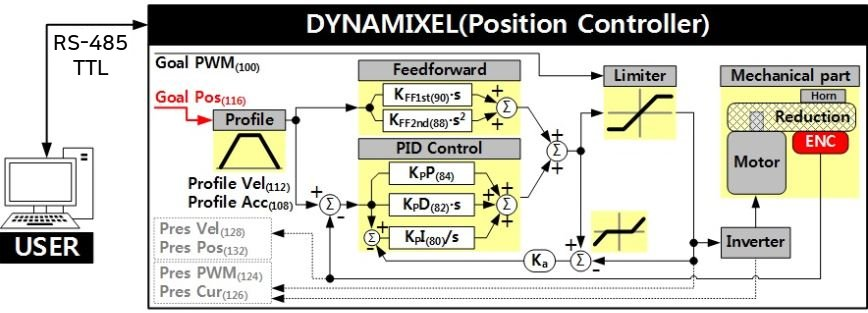
\includegraphics[width=0.6\textwidth]{Images/img_ch6/position_controller.jpg}} \quad 
    \subfloat[Velocity controller in Velocity Control Mode\label{fig:}]{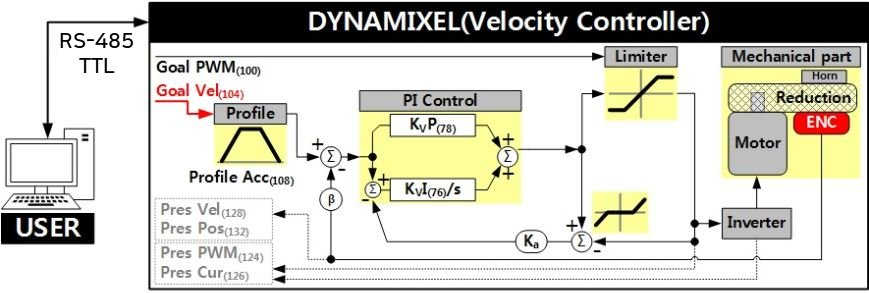
\includegraphics[width=0.6\textwidth]{Images/img_ch6/velocity_controller.jpg}}  
    \caption[Block scheme of DYNAMIXEL's position and velocity control mode]{Block scheme of DYNAMIXEL's position and velocity control mode}
    \label{fig:dynamixel_control}
\end{figure}

The DYNAMIXEL's closed loop controllers substitute the JTC in achieving the desired motion of the limbs, receiving the same command that was used in the simulation. 

In the transition from simulation to real system, controller gains adjustments are necessary, due to unexpected disturbances and mismatches in the estimated dissipative terms (friction and dumping of the joints).
For this reason, PID gains have been adapted, using again the \textit{root2end-end2root} approach, starting from a gain initialization equal to the values used for the JTC. 

Those modifications have been conducted during the single-limb testing, performed to test and validate the software update to control GRIEEL joints (discussed in the next chapter (\ref{sec:single_limb})).
The interface used to tune DYNAMIXEL controllers is represented in Fig.\ref{fig:dynamixel_GUI}, while the tracking performances after the tuning are reported in Fig.\ref{fig:dynamixel_tracking}.
By default, only proportional control is used, with a quick response but non-negligible steady-state error and overshoots, with the proposed gains instead, the steady-state error is eliminated and overshoots reduced.  

\begin{figure}[H]
    \centering  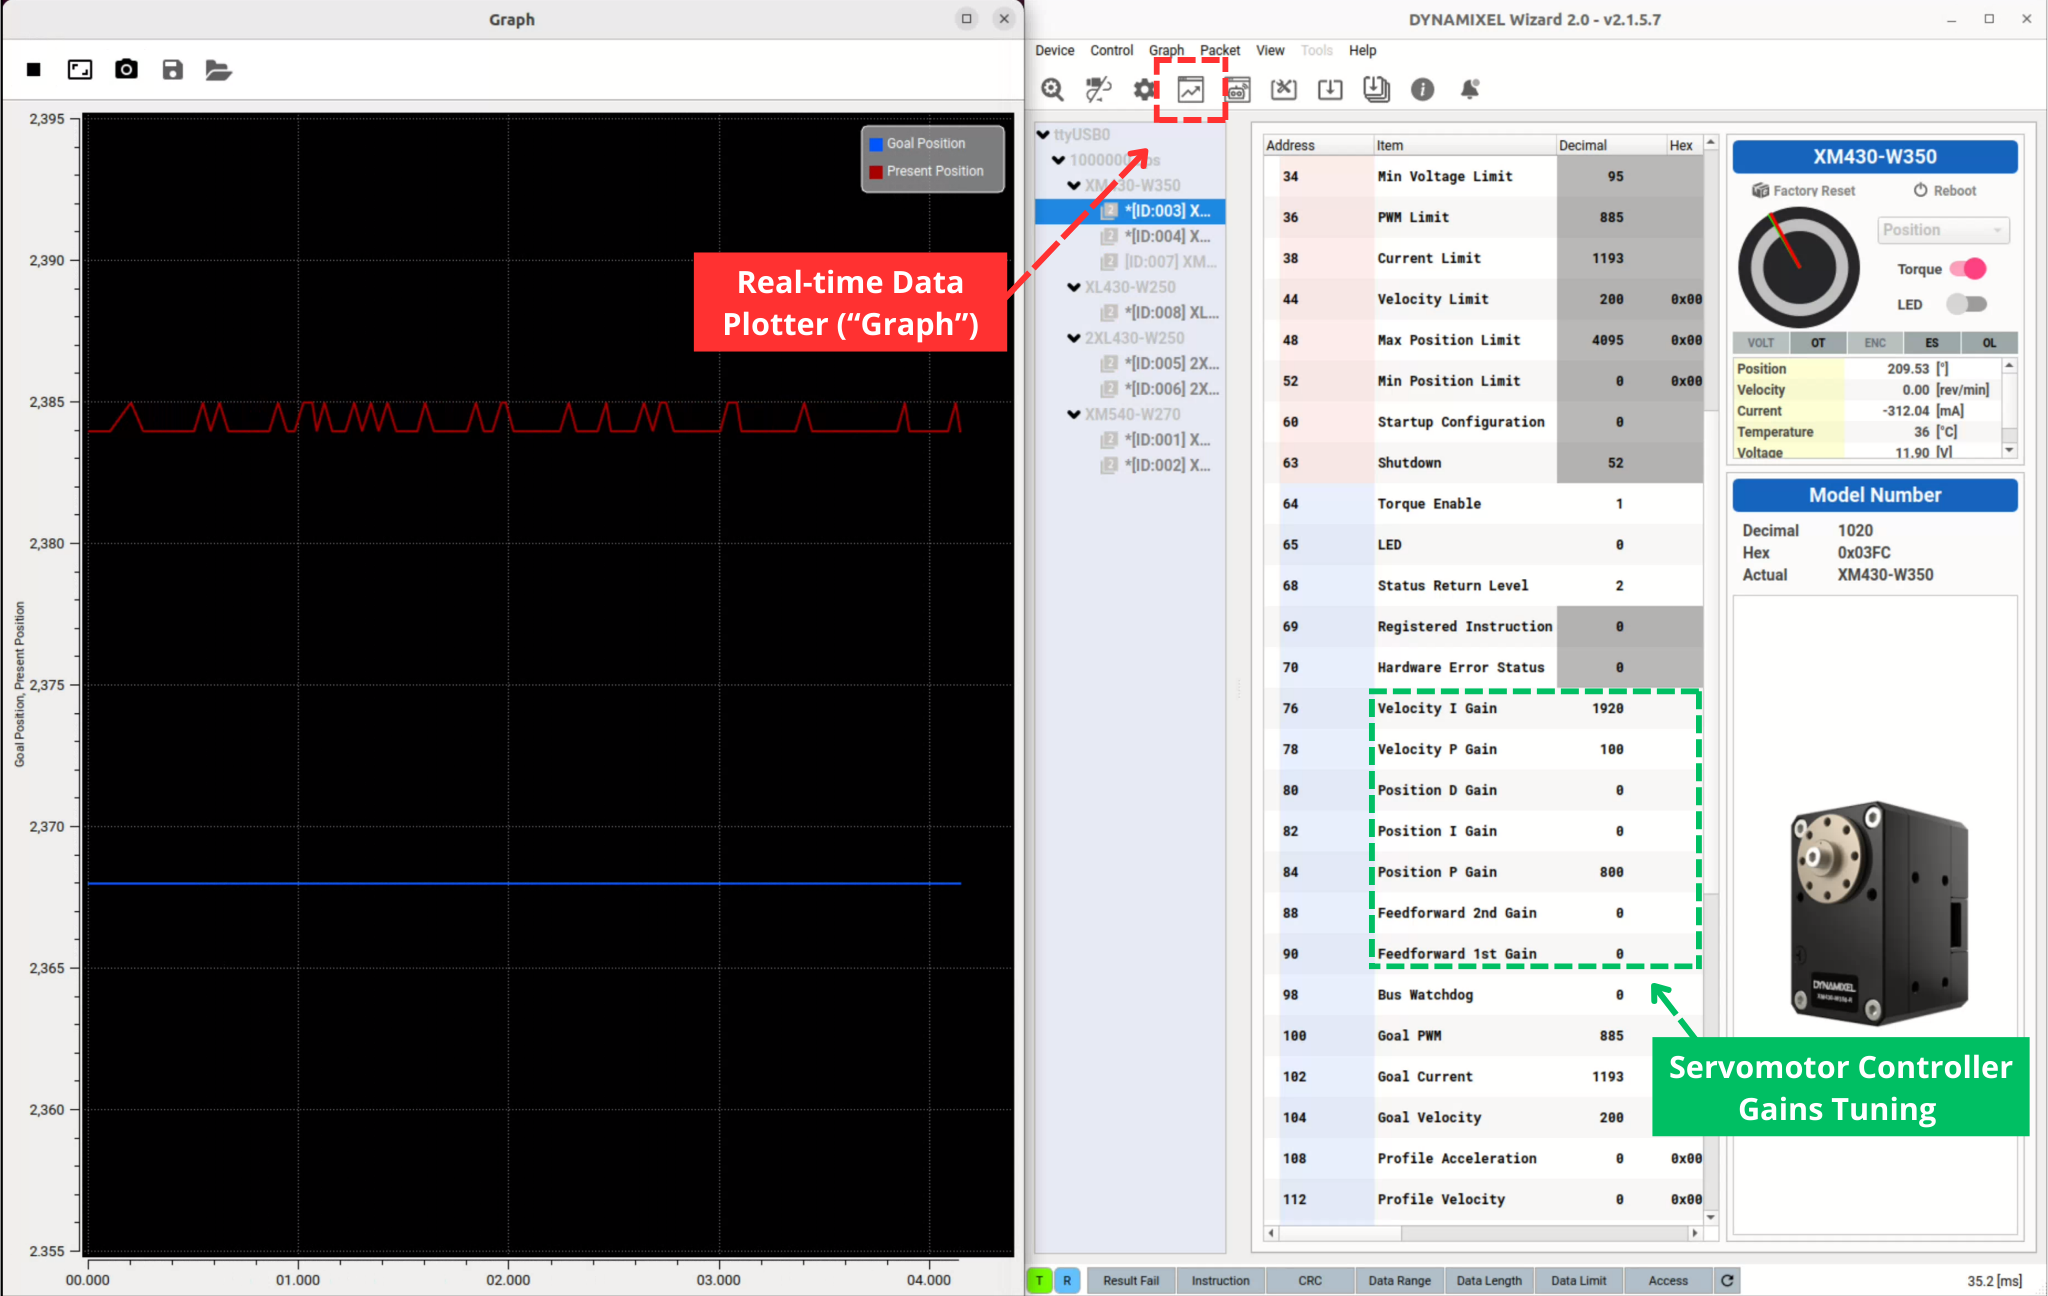
\includegraphics[width=0.85\textwidth]{Images/img_ch6/DynamixelUI.png}
    \caption{Dynamixel Wizard user interface, a tool to manage DYNAMIXEL motors.}
    \label{fig:dynamixel_GUI}
\end{figure}

Furthermore, when the four limbs were assembled with LIMBERO-GRIEEL, additional couplings between the limbs required small gains corrections.
The final tracking performances of the whole robot, achieved during the transformation, sequence are presented and discussed as part of the conclusions in chapter \ref{ch:chapter_eigth}.

\begin{figure}[H]
    \centering
    \subfloat{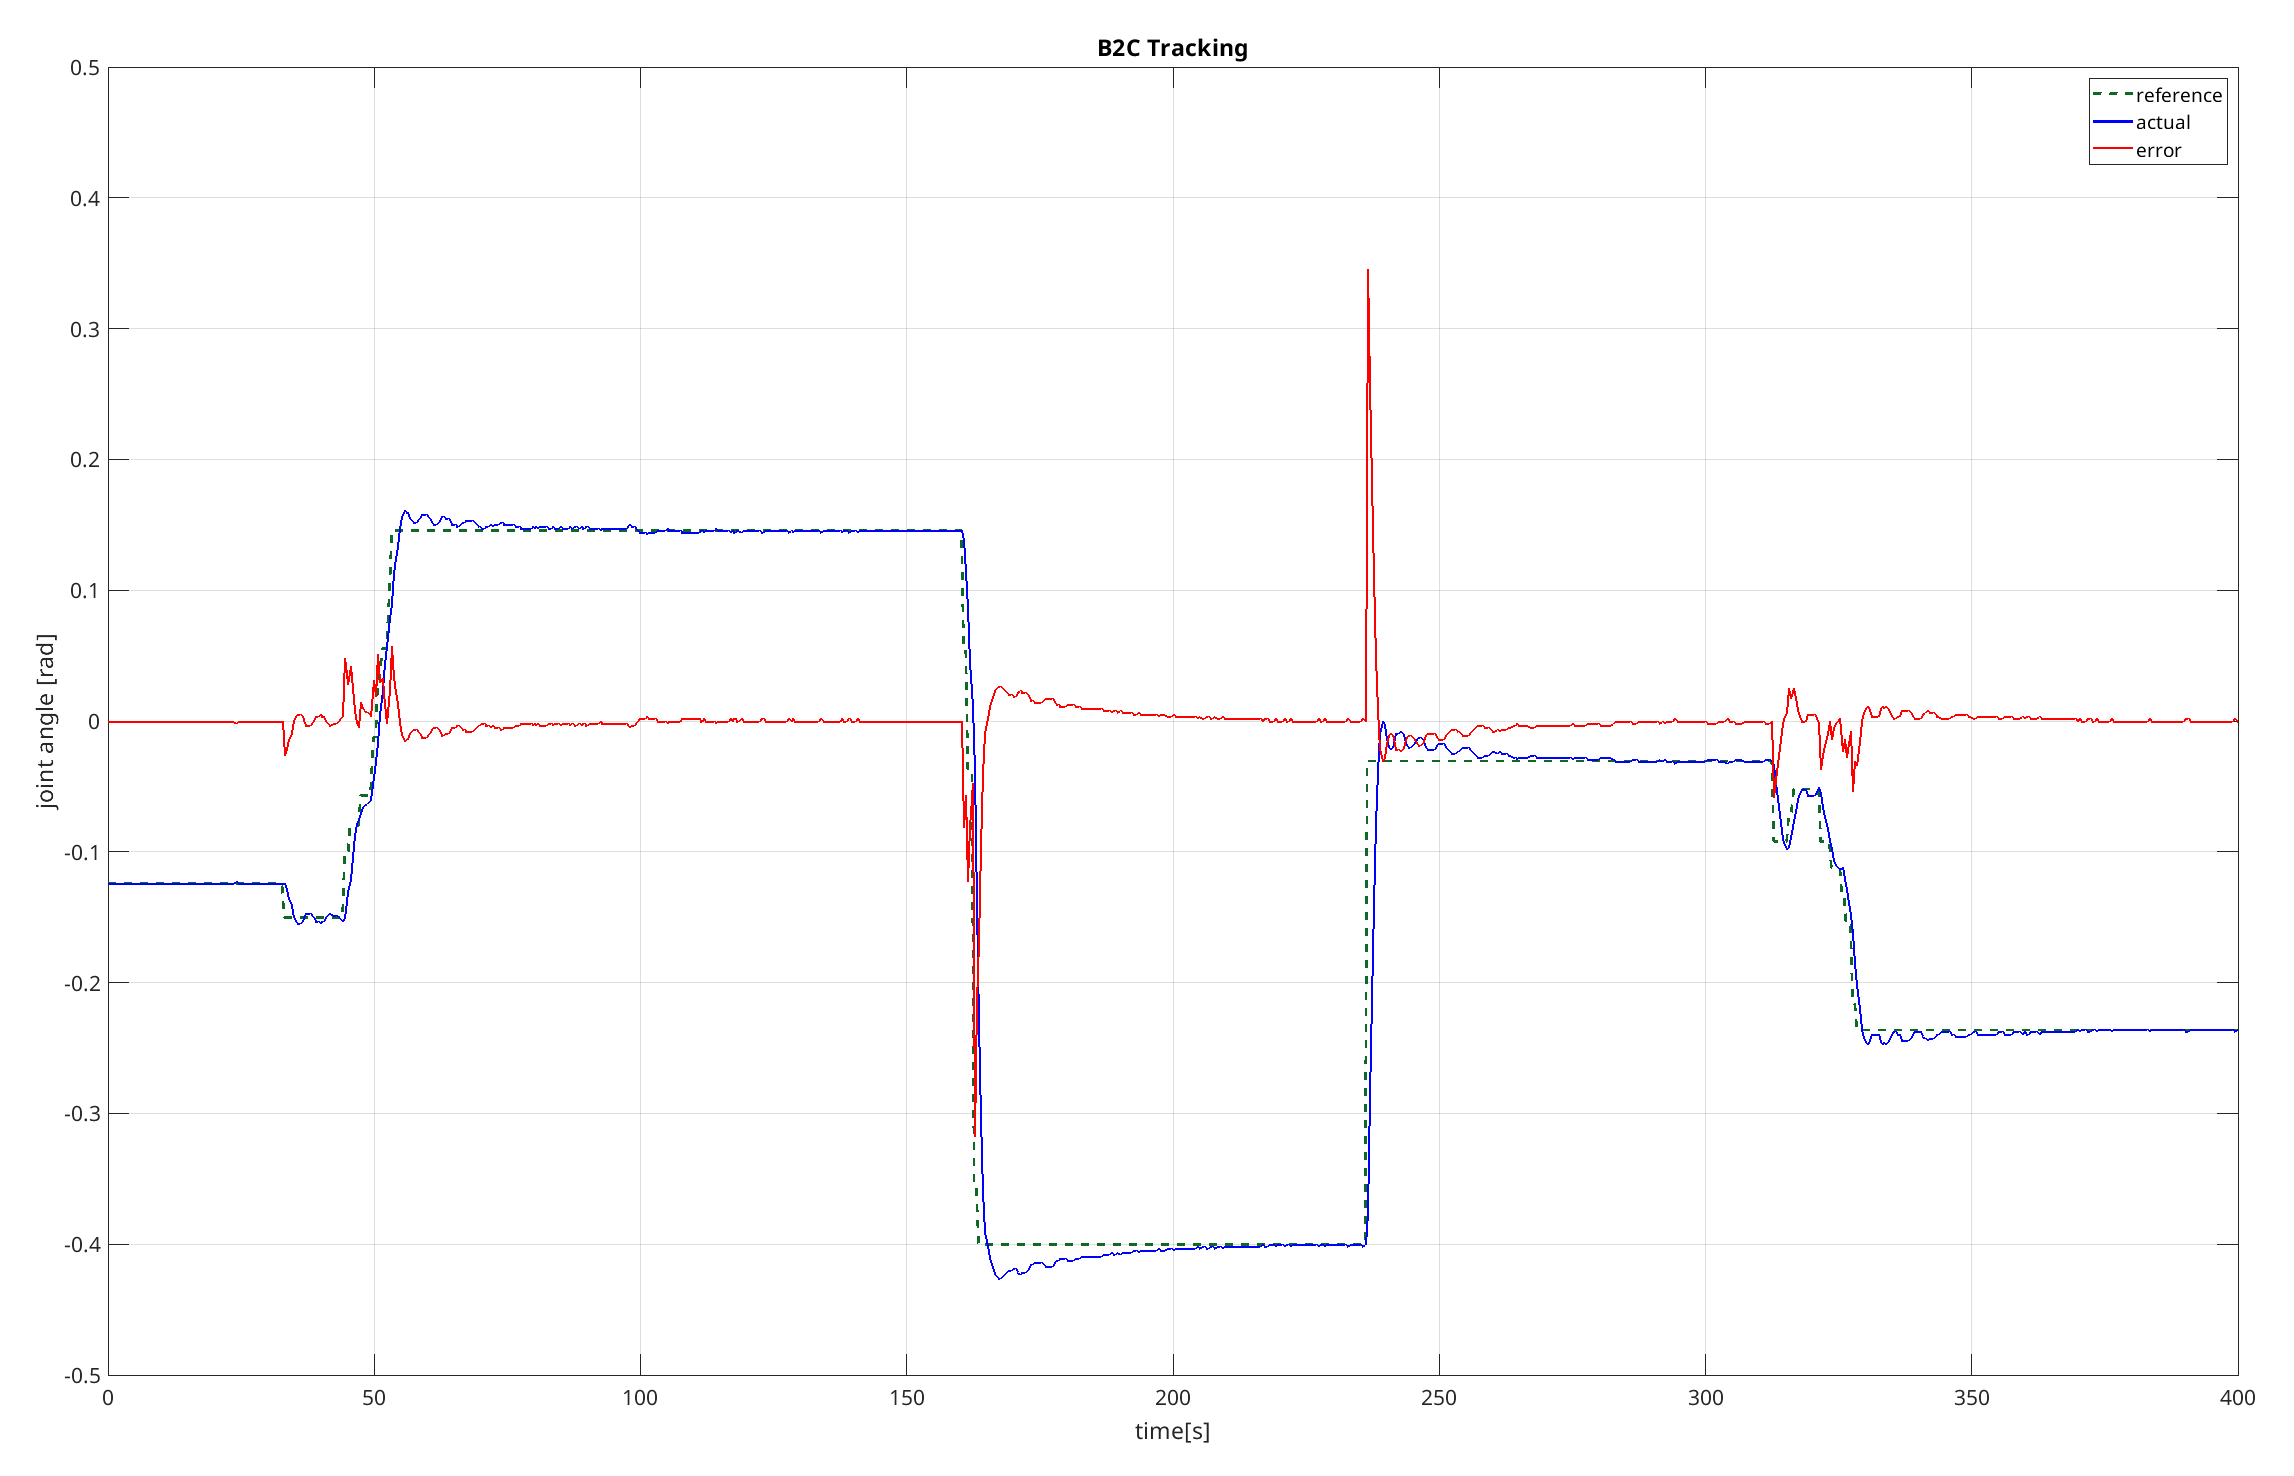
\includegraphics[width=0.5\textwidth]{Images/img_ch6/B2C_dynamixel.png}} \subfloat{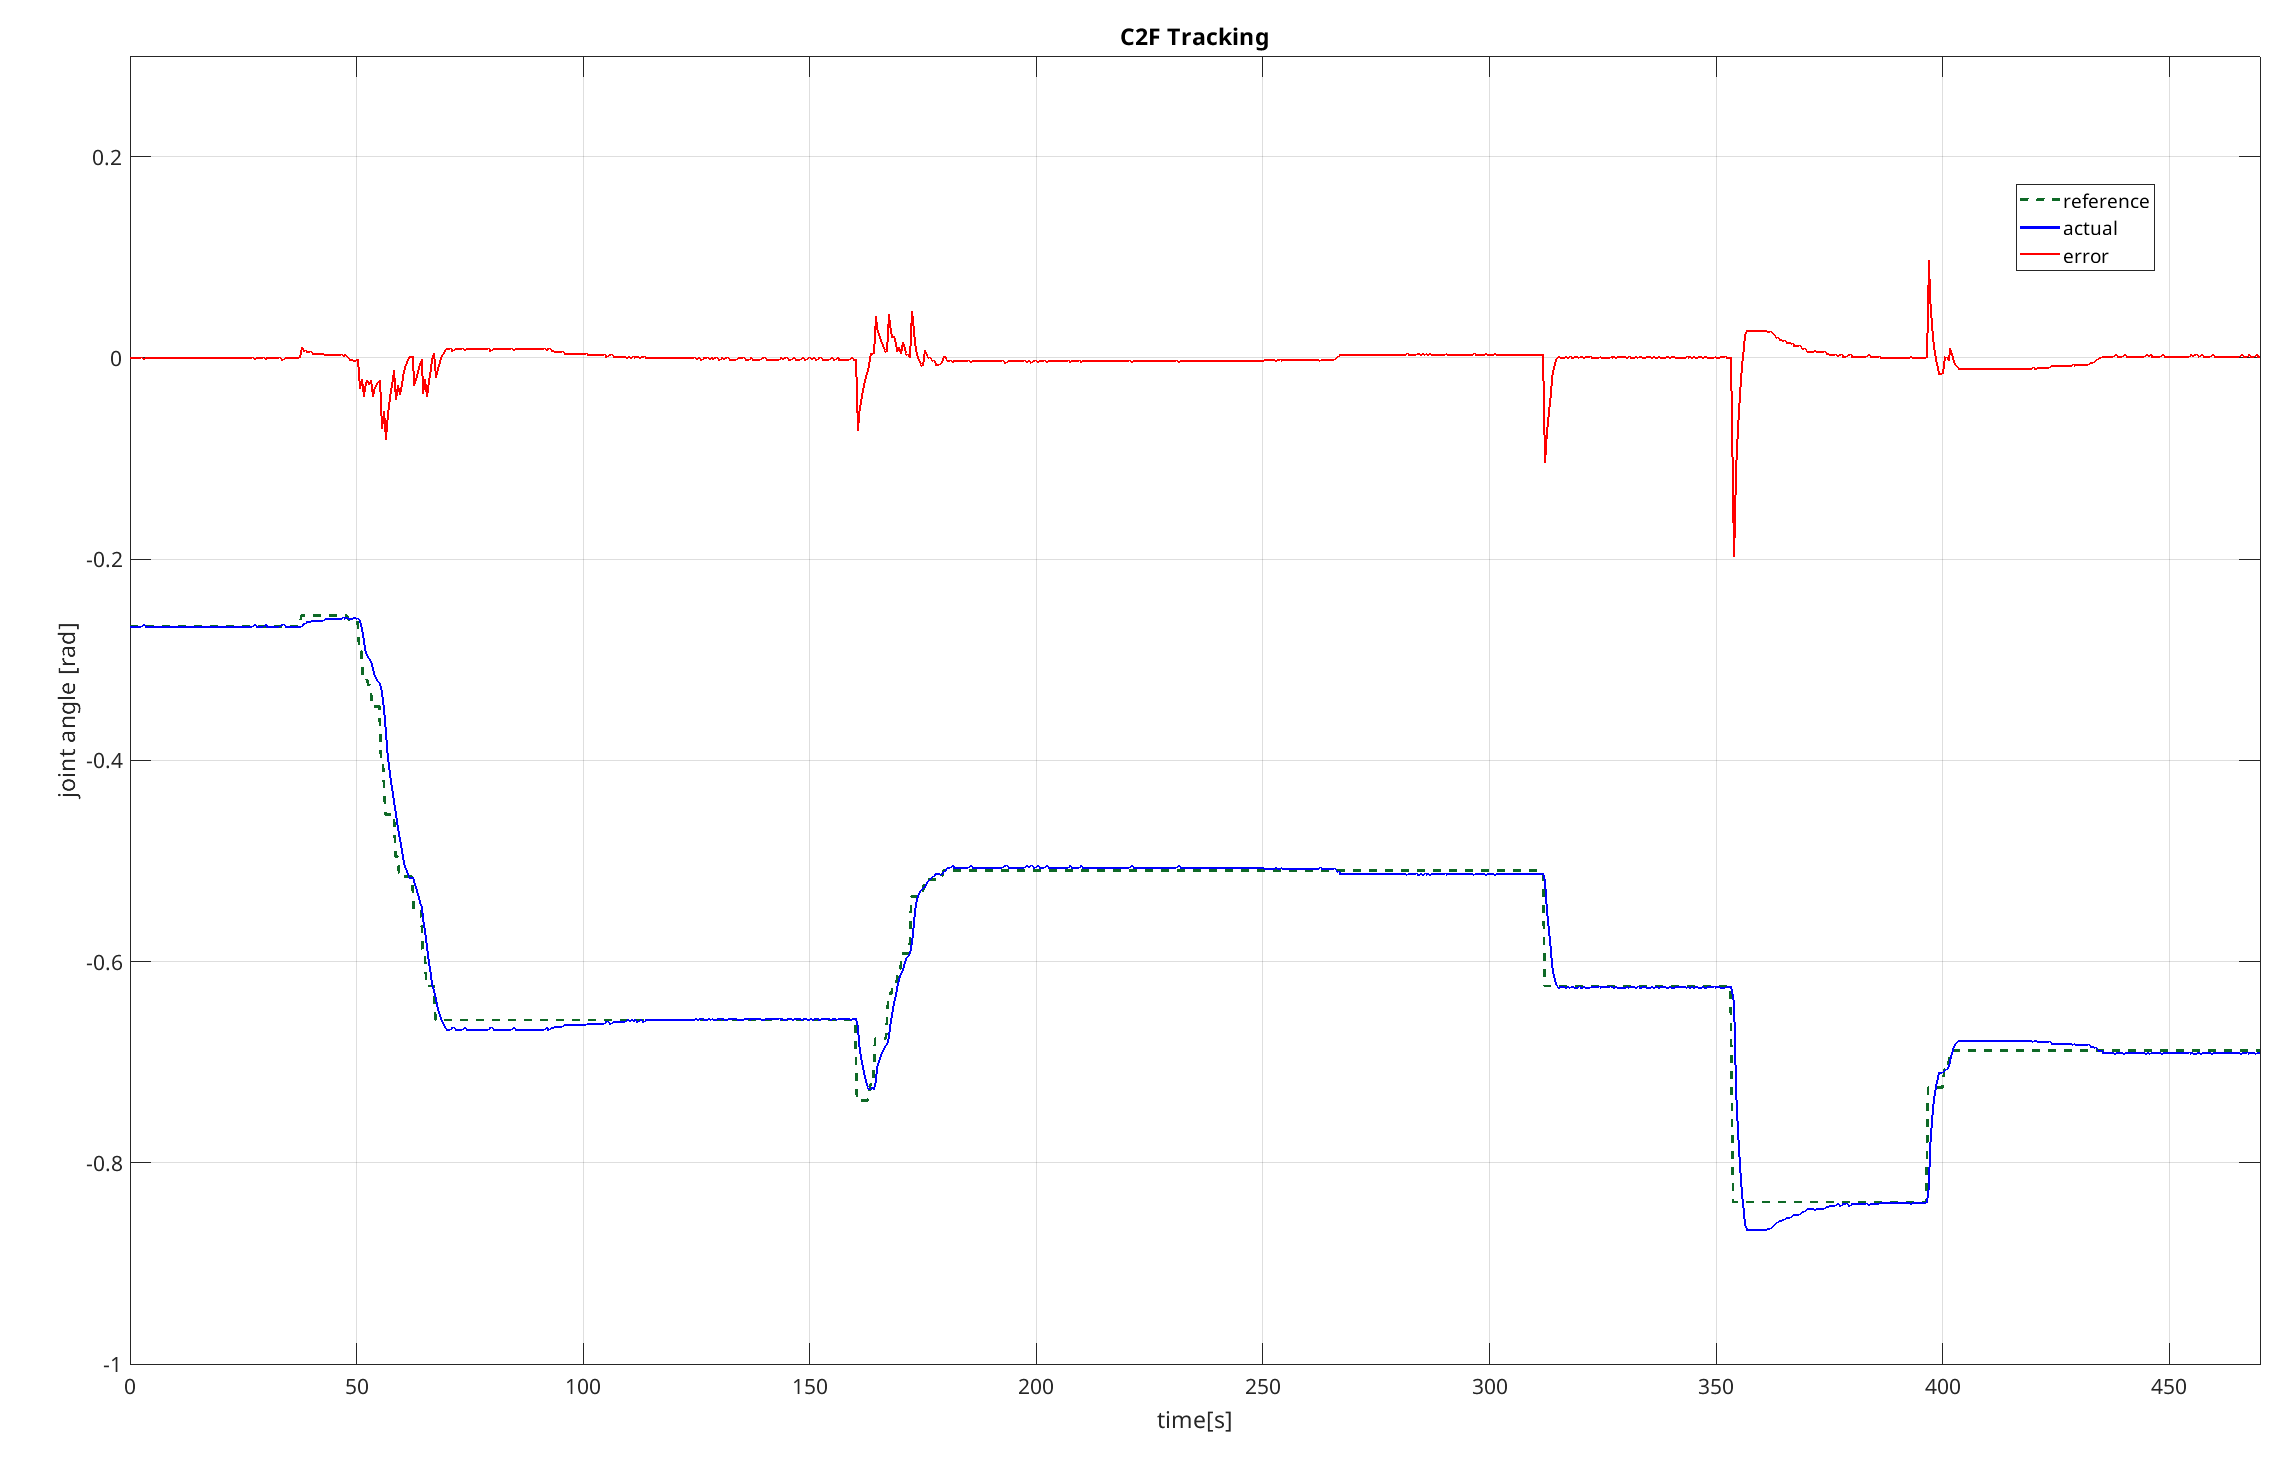
\includegraphics[width=0.5\textwidth]{Images/img_ch6/C2F_dynamixel.png}} \\
    \subfloat{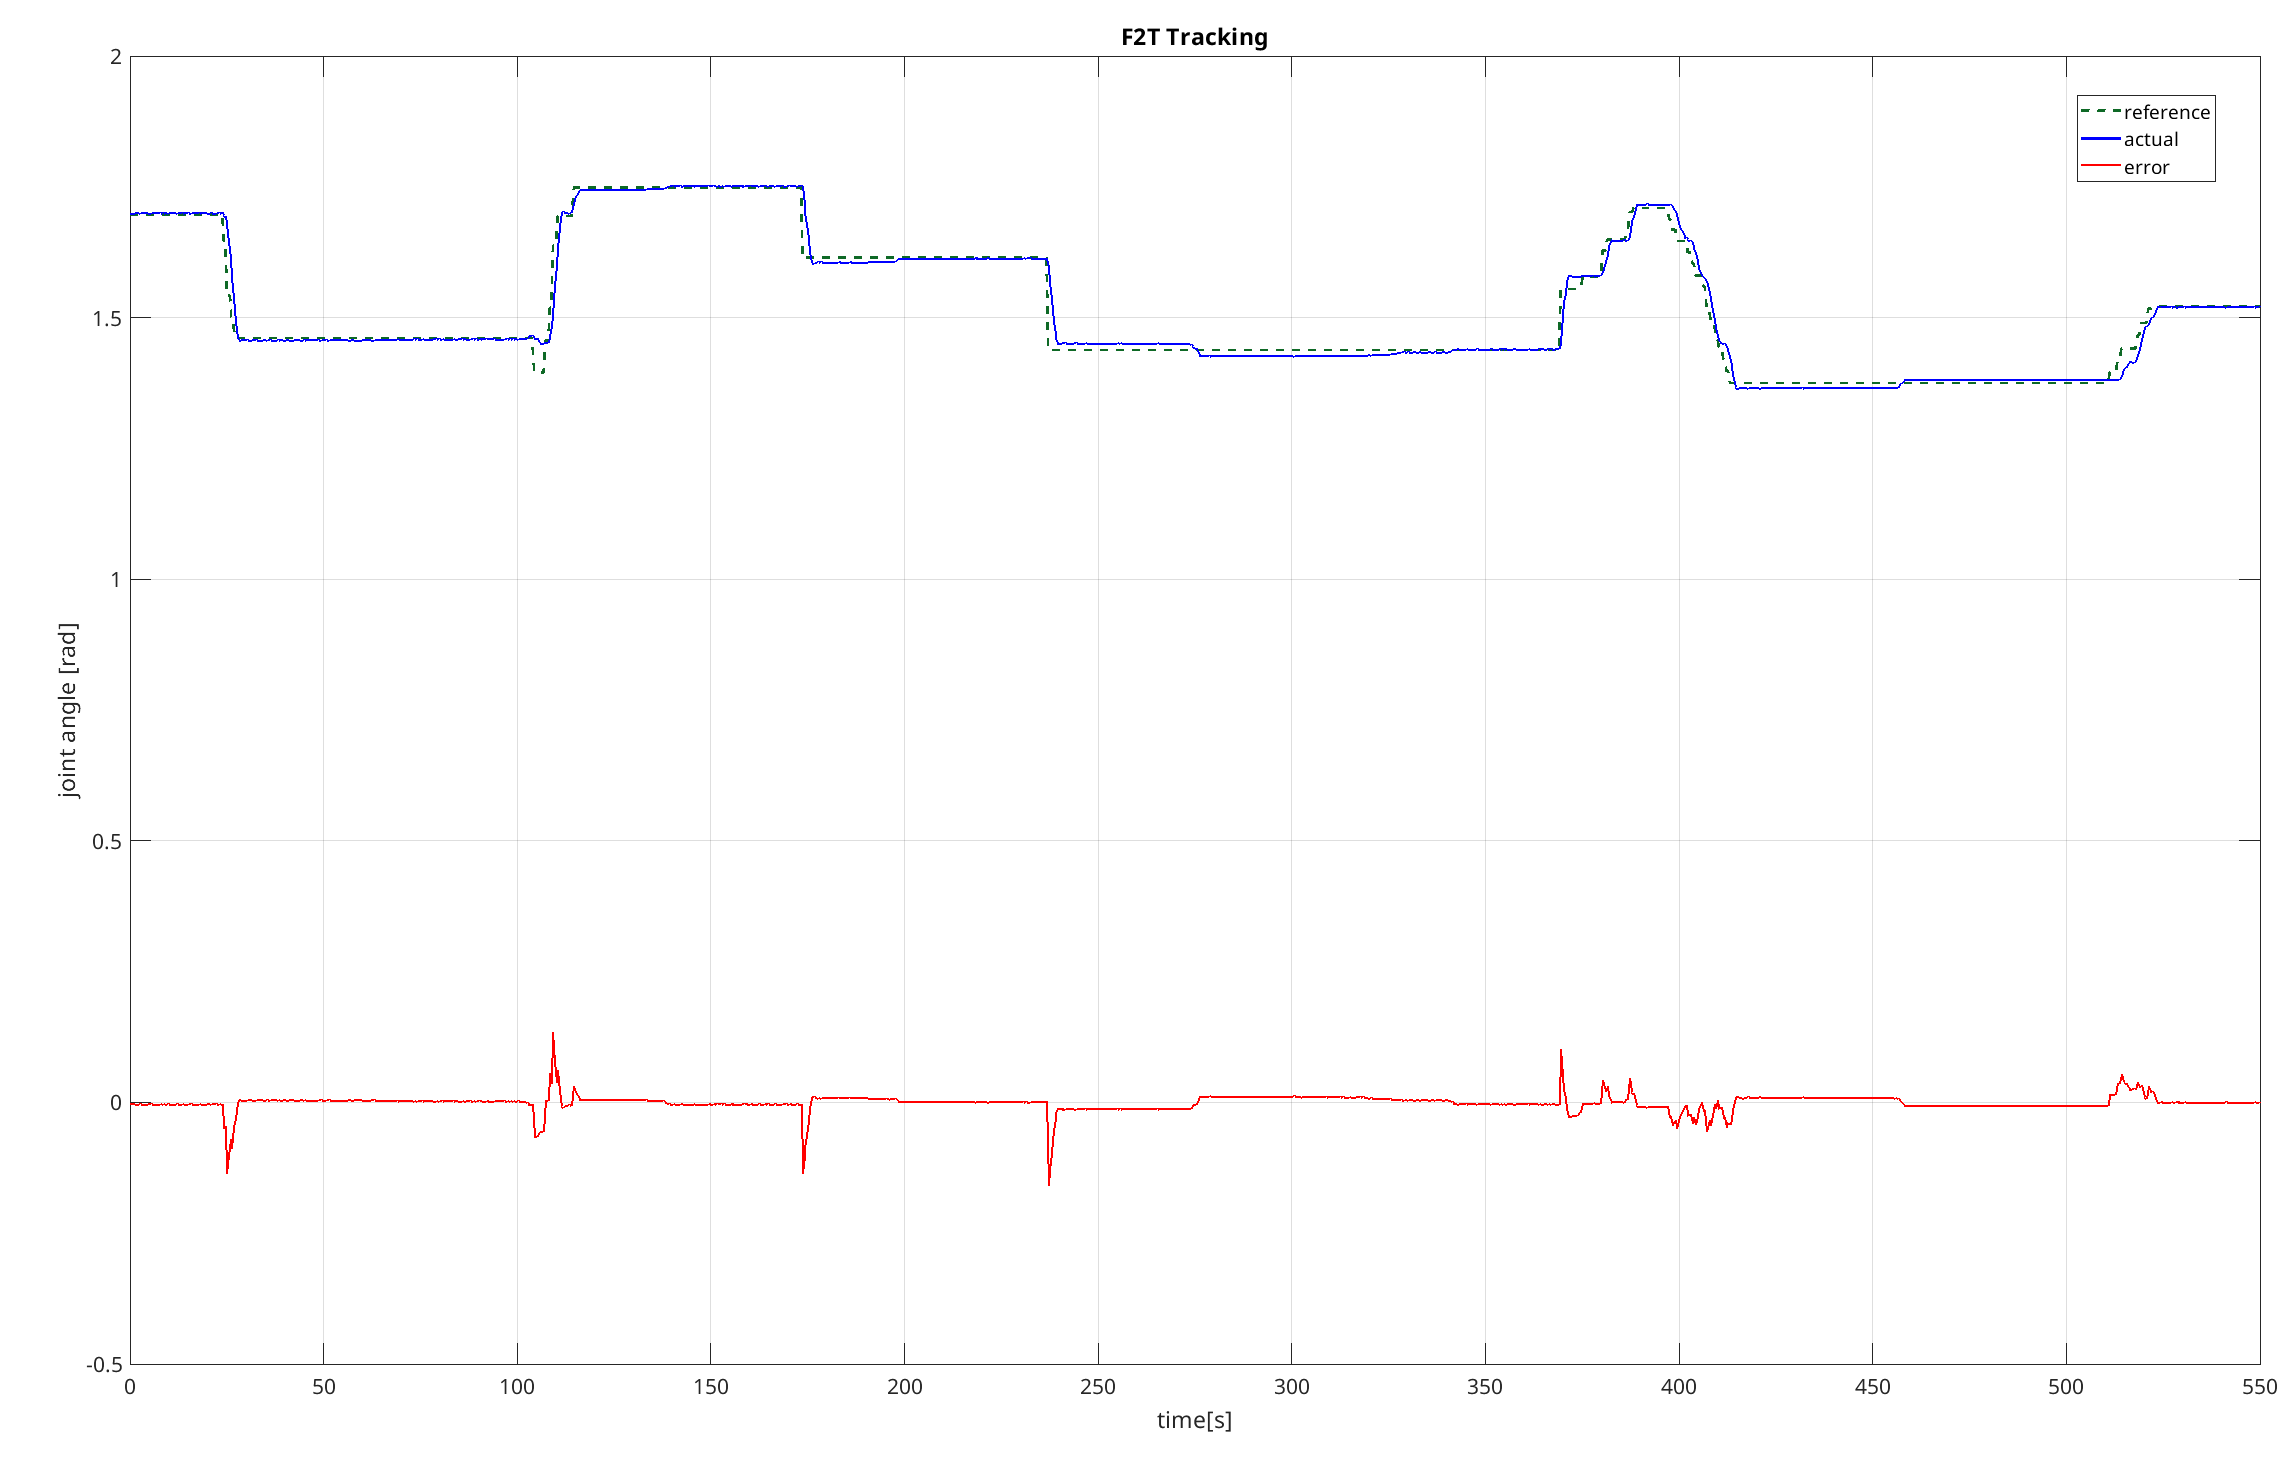
\includegraphics[width=0.5\textwidth]{Images/img_ch6/F2T_dynamixel.png}} 
\subfloat{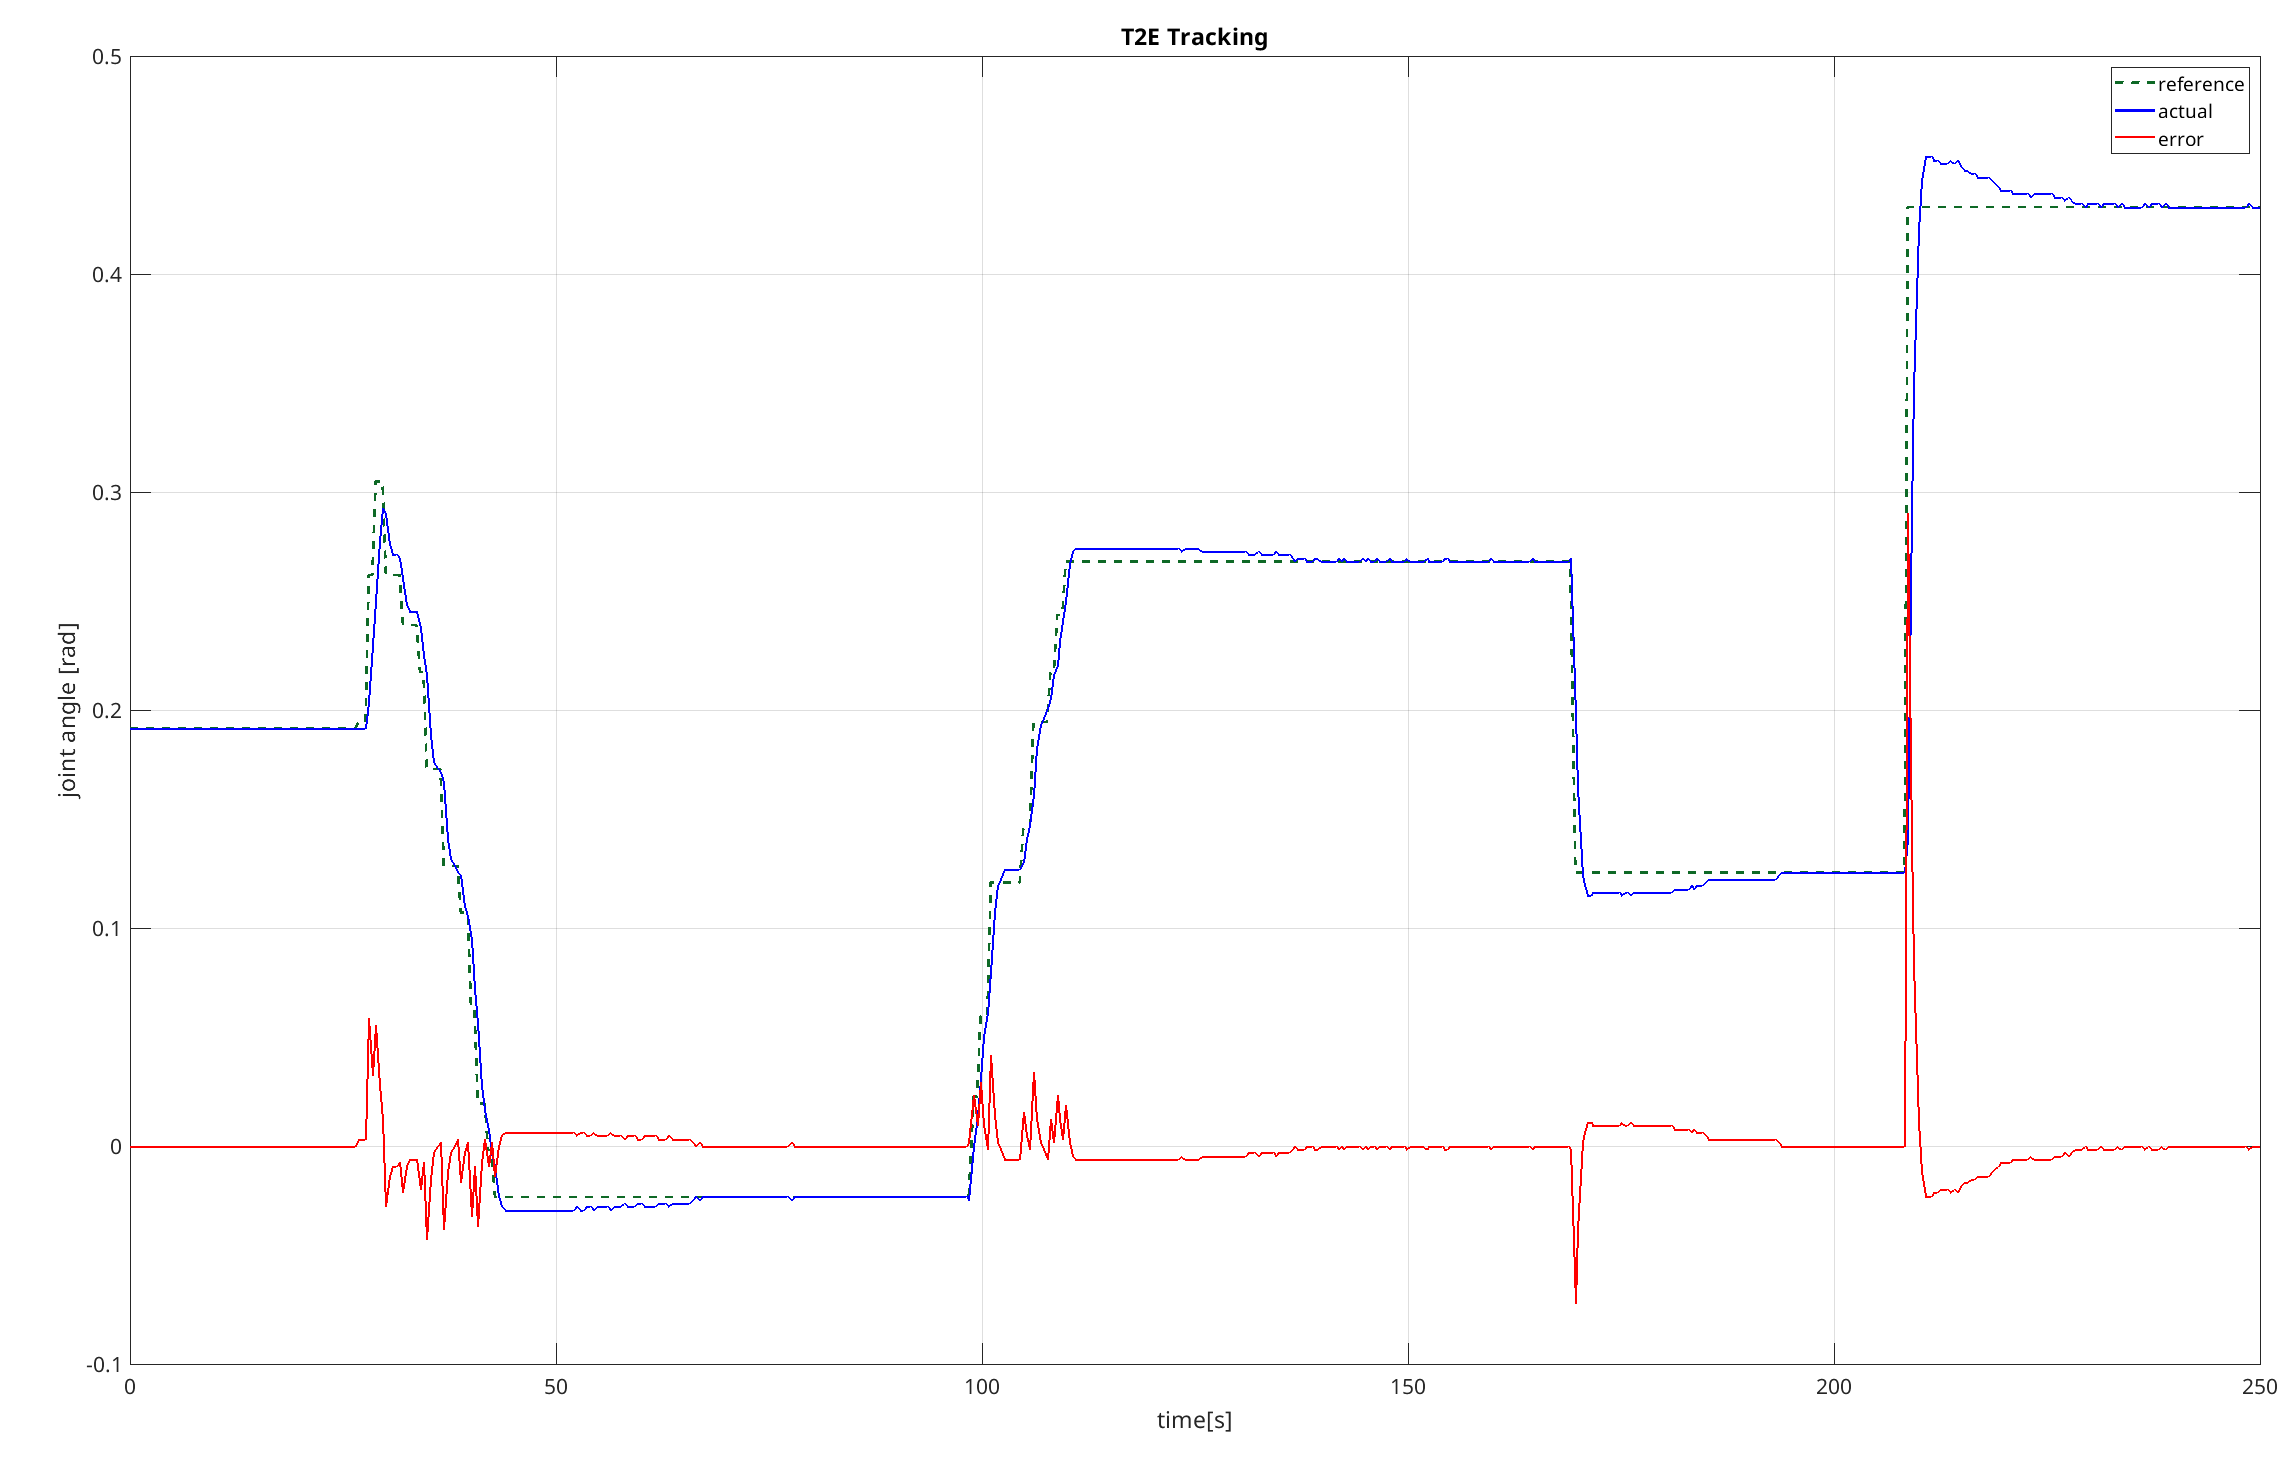
\includegraphics[width=0.5\textwidth]{Images/img_ch6/T2E_dynamixel.png}}  \\
    \subfloat{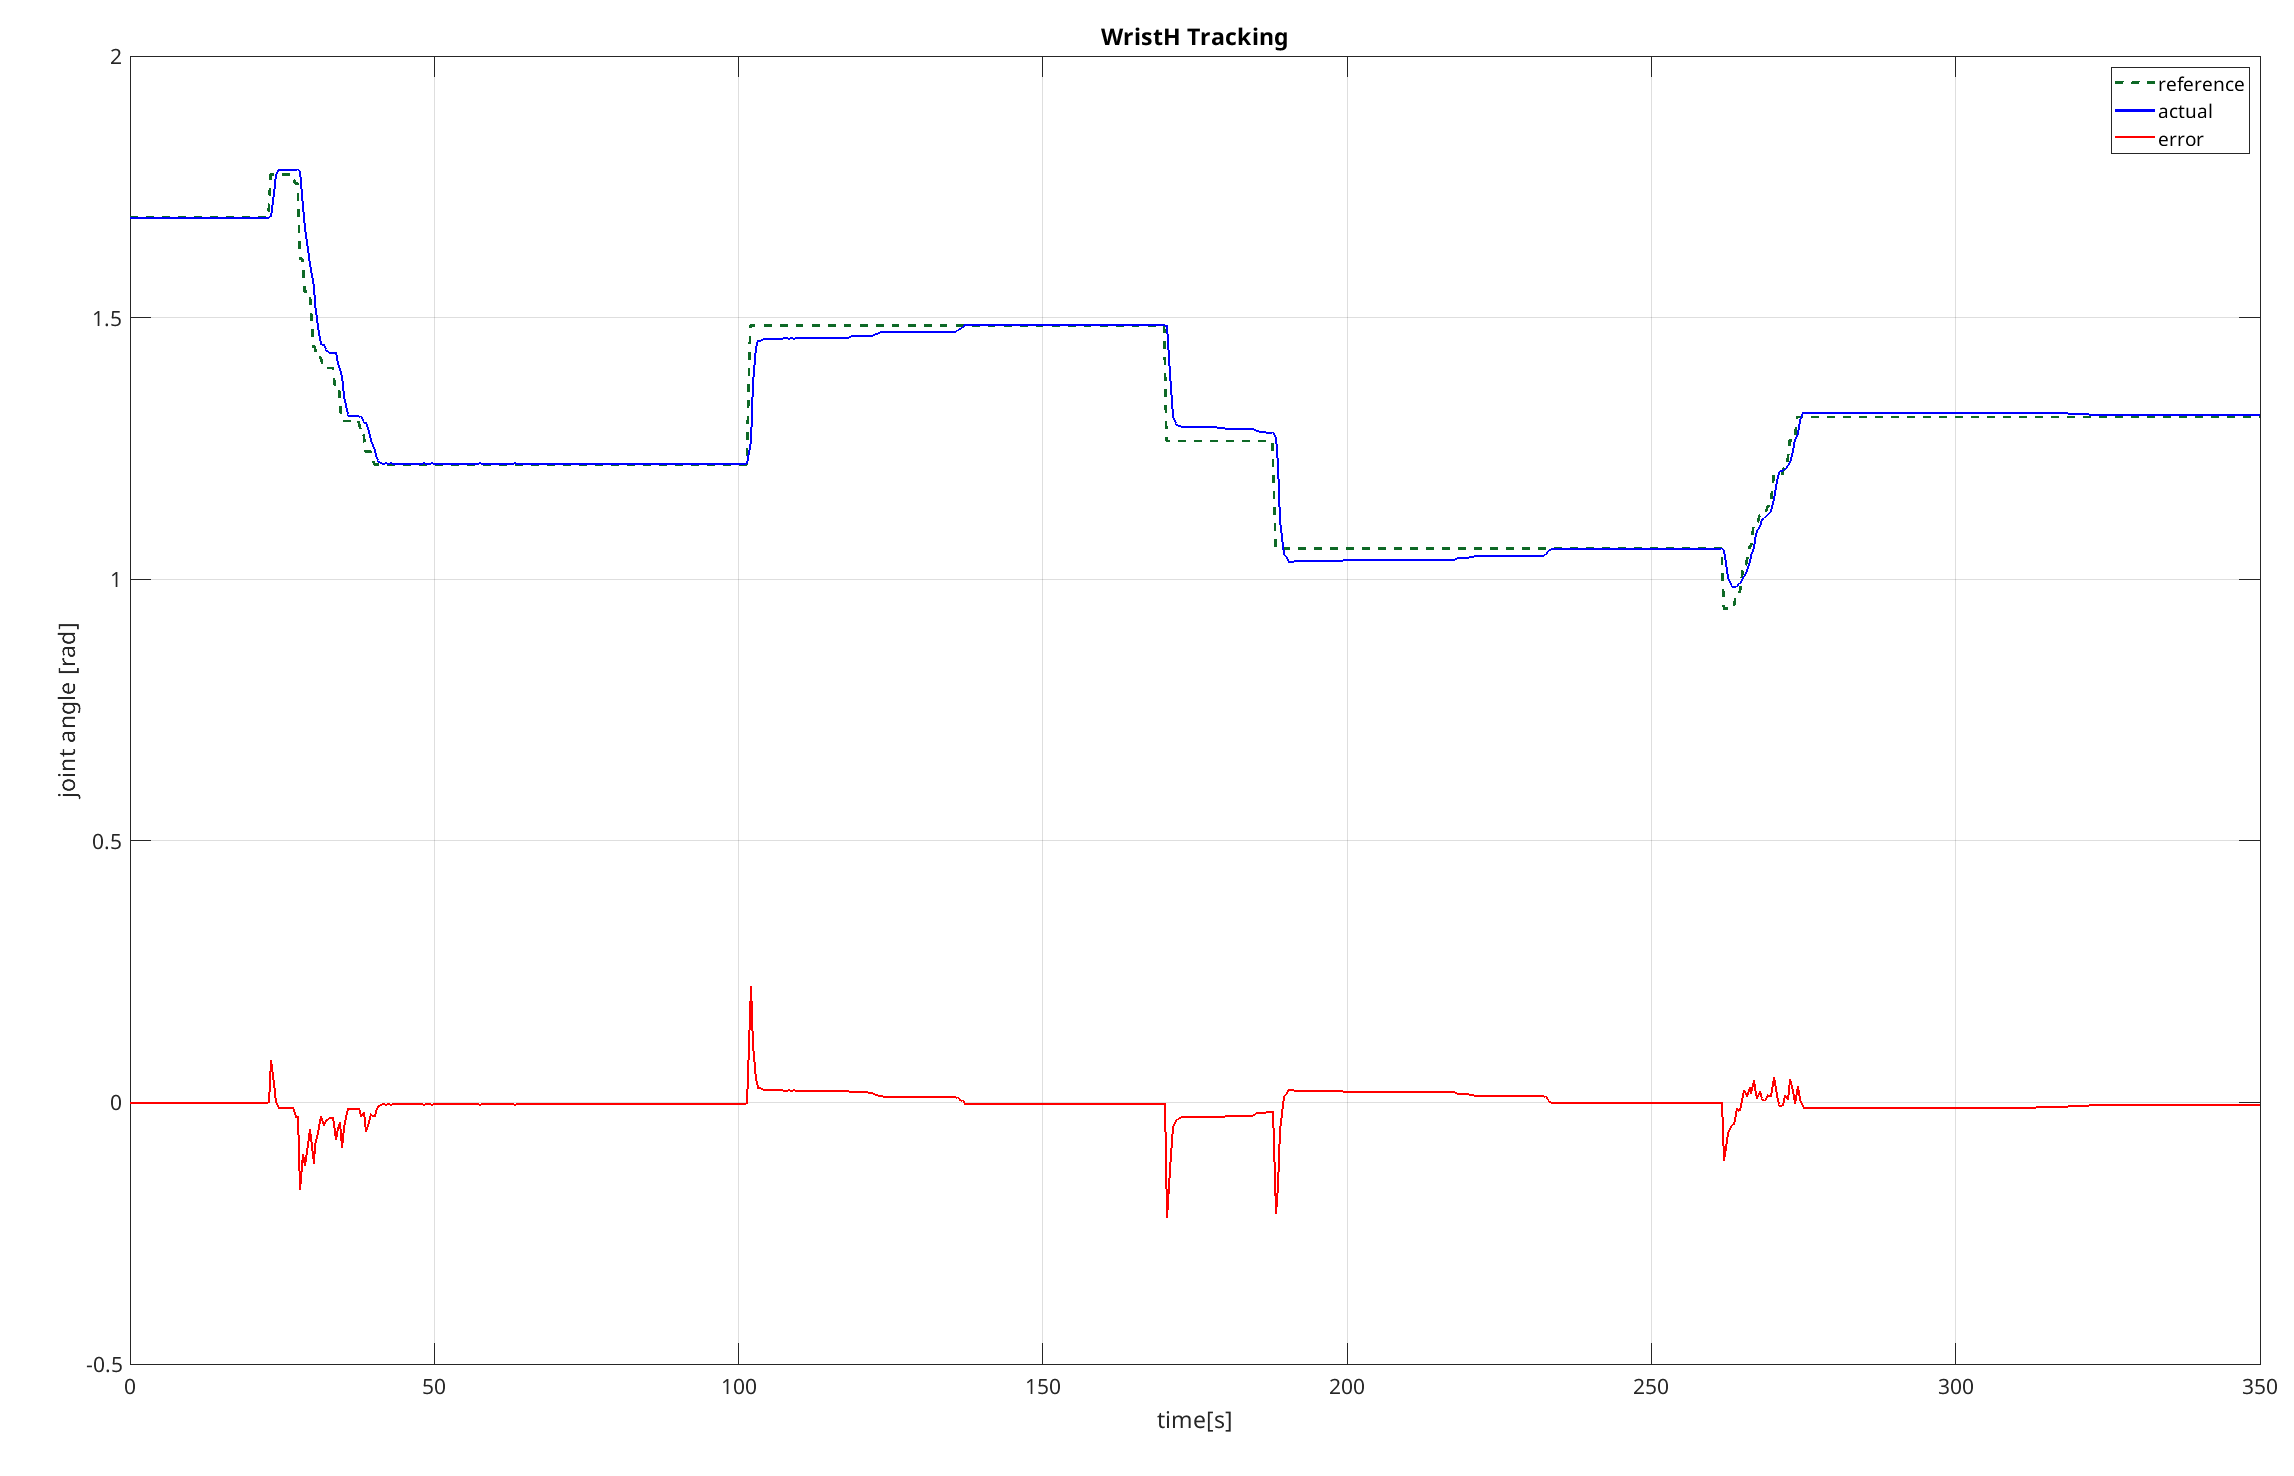
\includegraphics[width=0.5\textwidth]{Images/img_ch6/wristH_dynamixel.png}}  
    \subfloat{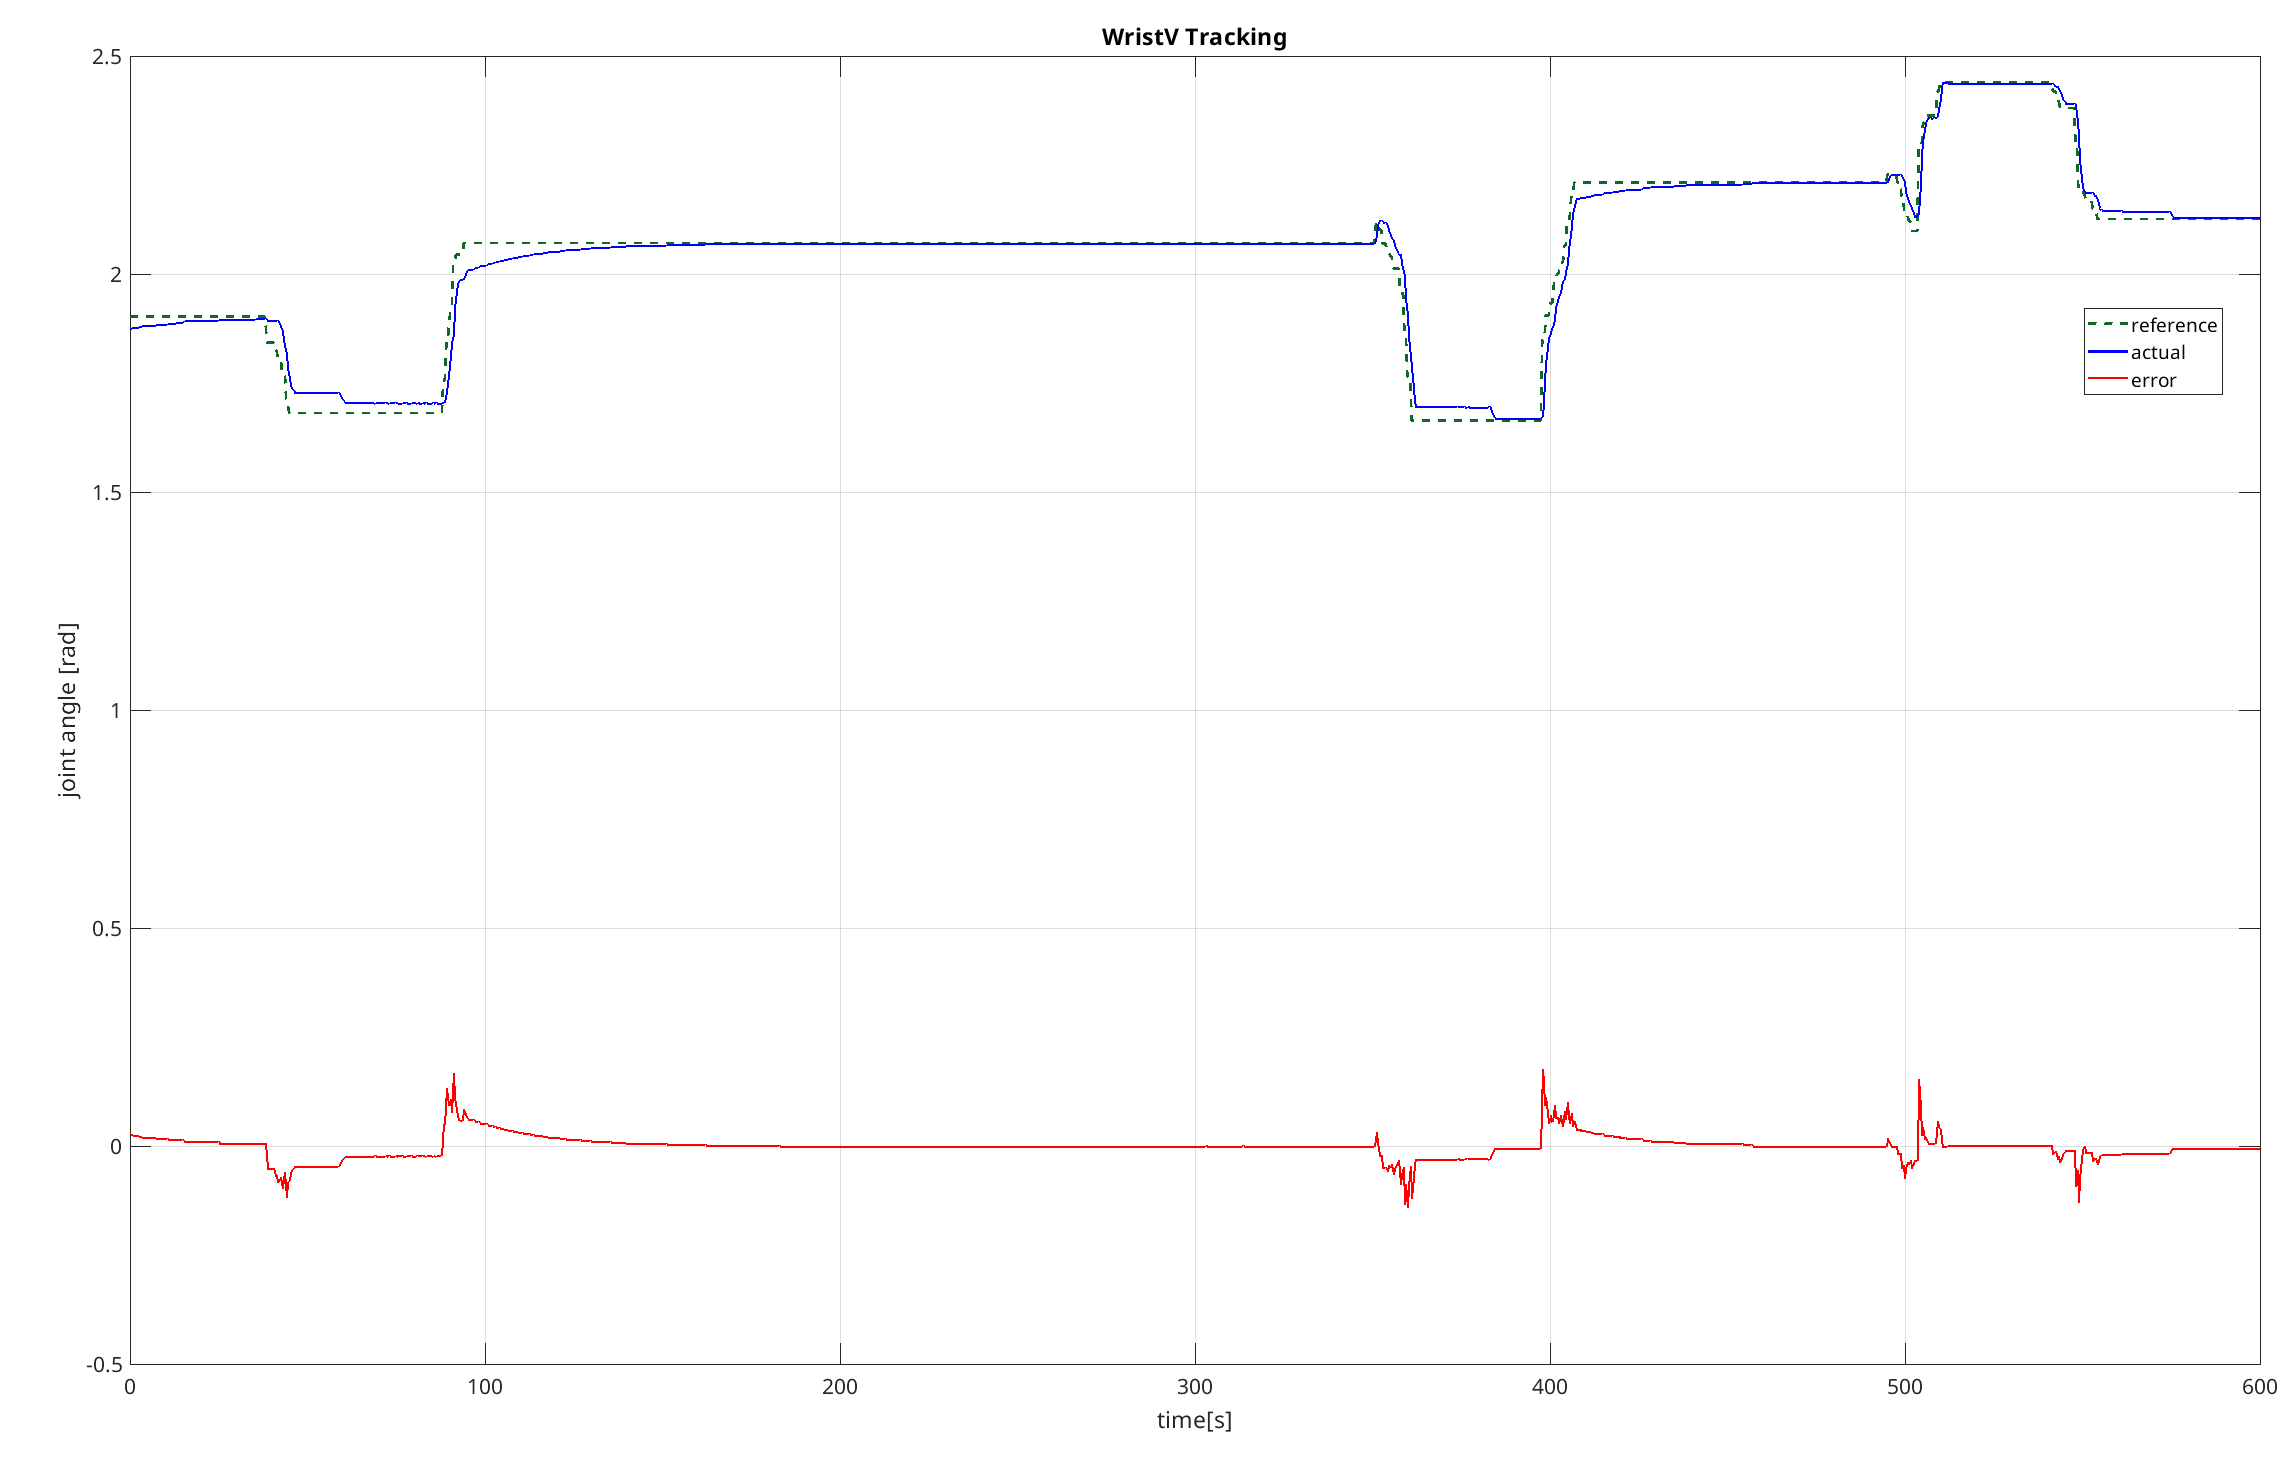
\includegraphics[width=0.5\textwidth]{Images/img_ch6/wristV_dynamixel.png}}  \\
    \caption[DYNAMIXELs joint trajectory tracking performance]{DYNAMIXELs joint trajectory tracking performance}
    \label{fig:dynamixel_tracking}
\end{figure}


\section{Indipendent Joint Controller}
\label{sec:IJC}

In the last phase of this research, without access to the hardware, it was necessary to set up a more reliable simulation environment where the transformation of the GRIEEL mechanism could be simulated. As discussed in section \ref{sec:simulation_description}, the choice has been a migration to the newer gazebo version. 
In this simulation environment, it has been possible to expose all joint torque signals and substitute the JTC with closed-loop independent joint controllers (IJCs), implemented from scratch. The new control scheme of each joint is represented in Fig.\ref{fig:IJC_scheme}, it uses a P+PI scheme as the one described in section \ref{sec:IndipendentJointControl}, with an additional reference pre-filter, and anti-wind up based on the back-calculation algorithm\cite{AntiWindUpBackCalculation1}\cite{AntiWindUpBackCalculation2}\cite{AntiWindUpBackCalculation3}\cite{AntiWindUpBackCalculation4}.
Furthermore, in the design of the independent joint controller for the driving motor, a switching controller gains is considered for the driving motor, which is controlled directly at velocity level with a PI controller. For this research, when in gripper mode, the driving motor is kept fixed by the transmission system and the servomotor internal controller, and the proportional and integral gain is set to 0 with a re-initialization of the integrator value. When transforming into wheel mode, instead,  the gains are set to a non-null value (and the integrator is re-initialized)( to control driving locomotion. 

\begin{figure}[H]
    \centering
    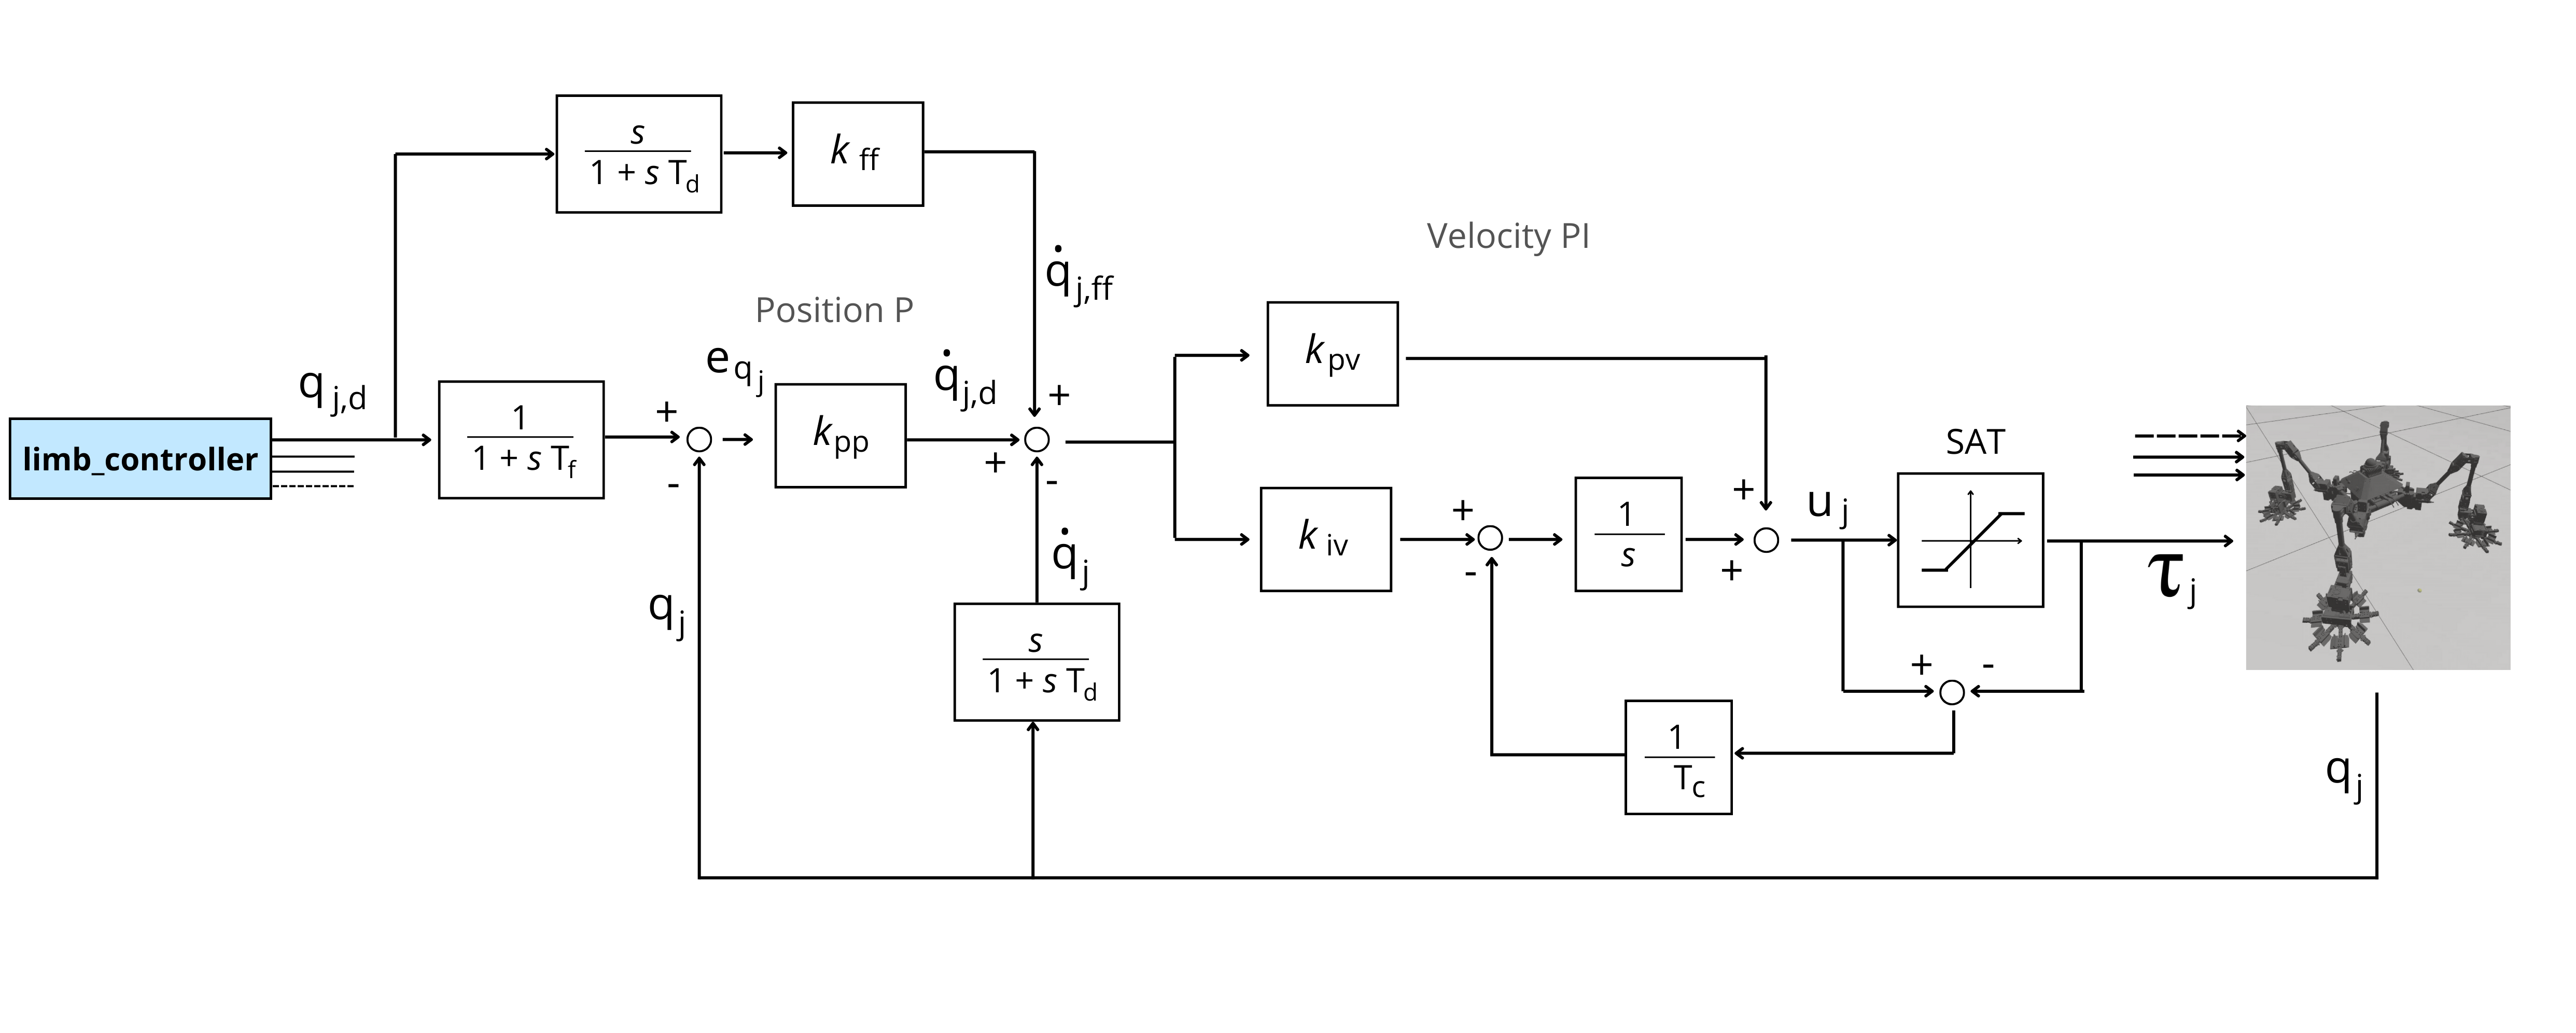
\includegraphics[width=0.95\textwidth]{Images/img_ch6/IJC_limbero.png}
    \caption{Block scheme of each joint's IJC, integrated into ROS2 architecture by discretization.}
    \label{fig:IJC_scheme}
\end{figure}

In this new environment, the tuning has been conducted on a single LIMBERO-GRIEEL limb, with a model-based approach instead of an empirical one. As introduced in section \ref{sec:matlab}, the model identification has been carried out in MATLAB. 

The final model is a decoupled joint dynamic, such as the one in \ref{sec:DecoupledDyn}, described by Equation \ref{eq:DecoupledManipulatorEoM}.
However, to take into account the dual nature of the limbs, both a swing and contact model have been defined, considering that when the limb touches the ground it "manipulates" the base (remember the multi-limbed duality with cooperative arms \ref{sec:multi_limb_coopmanipulators}), while if not in contact behave as a robot arm. With this dual, the decoupled dynamic inertia is considered an average of the two models, ensuring more reliability rather than modeling only a swing phase.

The steps of the model identification procedure are summarized here: 
\begin{enumerate}
    \setlength\itemsep{-0.7em} 
    \item Convert the limb simulation model (URDF) to a serial link DH model, referred to as \textbf{limb-DH}, through the required frame transformations. 
    \item Transform dynamic properties (inertia tensor and CoM) of the URDF in the new DH frames
    \item Define the dual model when in contact, by inverting the joint sequence, and considering the robot base as the "tool". 
    \item Identify each joint average inertia from the inertia matrix of the two models, considered in multiple feasible limb configurations.
    \item Derive the equivalent decoupled joint models for all limb joints, referred to as \textbf{limb-IJs}. Where reduction ratio and motor inertia are taken from the online data sheet of DYNAMIXELs. 
\end{enumerate}

From the steps above, both a complete limb model for simulation  (\textbf{limb-DH}) and decoupled joint models (\textbf{limb-IJs}) are available in Matlab.
Finally, limb-IJs are used for controller tuning, while limb-DH for testing the performance of the controllers in a more realistic dynamical system. 

Using the limb-IJs model, classical control theory approaches such as loop shaping are used to derive the gains of the P+PI controllers, ensuring the requirements defined in terms of position/velocity cut-off frequency \cite{ControlTheory}. 
Then limb-DH is imported in a Simulink scheme with a trajectory generator and the implementation of the IJCs, and possible gains correction are considered. 
Furthermore, when porting the controller implementation in ROS2 using Gazebo Harmonic, additional adjustments of those gains are necessary to counteract additional dissipative effects and simulation limitations. 

The final results are discussed as part of the simulation results \ref{sec:sim_result_harmonic}. 









